\section{Diagramma Concettuale}\label{concettuale}
\begin{figure}[ht]
    \centering
    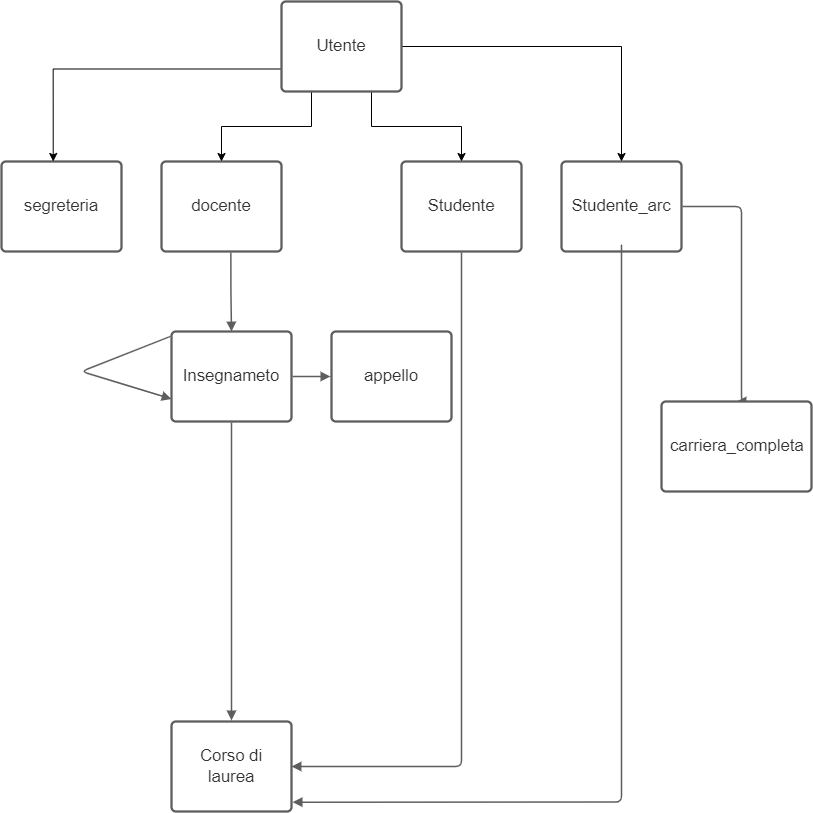
\includegraphics[width=0.5\linewidth]{images/concettuale-1.png}
    \caption{Prima versione del diagramma concettuale}
    \label{fig:concettuale1}
\end{figure}
Iniziamo a sviluppare il diagramma concettuale partendo da ciò che possiamo dedurre a una prima lettura della consegna, sapremo che avremo le  seguenti entità:
\begin{itemize}
    \item Utente:
    \begin{itemize}
        \item Segreteria
        \item Docente
        \item Studente
        \item Studente Archiviato
    \end{itemize}
    \item corso di laurea 
    \item Insegnamento
\end{itemize}

\subsection{Utenti}
Per prima cosa concentriamoci su utenti i quale si trovano in una gerarchia e necessità una ristrutturazione:

procederemo con una ristrutturazione verso il basso dove quindi ci assicureremo che ogni entità figlia sia indipentente
\subsection{Insegnamenti}
non necessità di particolari ristrutturazioni se non una specificazione che la relazione con se stessa definisce la propedeuticità  e si tratta di un n-n
\subsection{Corso di Laurea}
non necessità ristrutturazioni
\subsection{Studente}
non necessità ristrutturazioni
\subsection{Appello}
Appello necessita di una grande ristrutturazione in quando necessità un associazione a studente e l'aggiunta di una tabella che permettà l'iscrzione agli studenti che chiameremo sostiene (\ref{sostiene})
\subsection{Archivio}
Per quanto riguarda la gestione della tabella carriera completa segue una ristruttuazione in linea con la struttura esposta nella sezione \ref{archivio}

\subsection{Aggiornamento Diagramma}
applicando quindi le ristrutturazioni sopra citate possiamo illustrare il nuovo diagramma concettuale in figura \ref{fig:concettuale2}
\begin{figure}[ht]
    \centering
    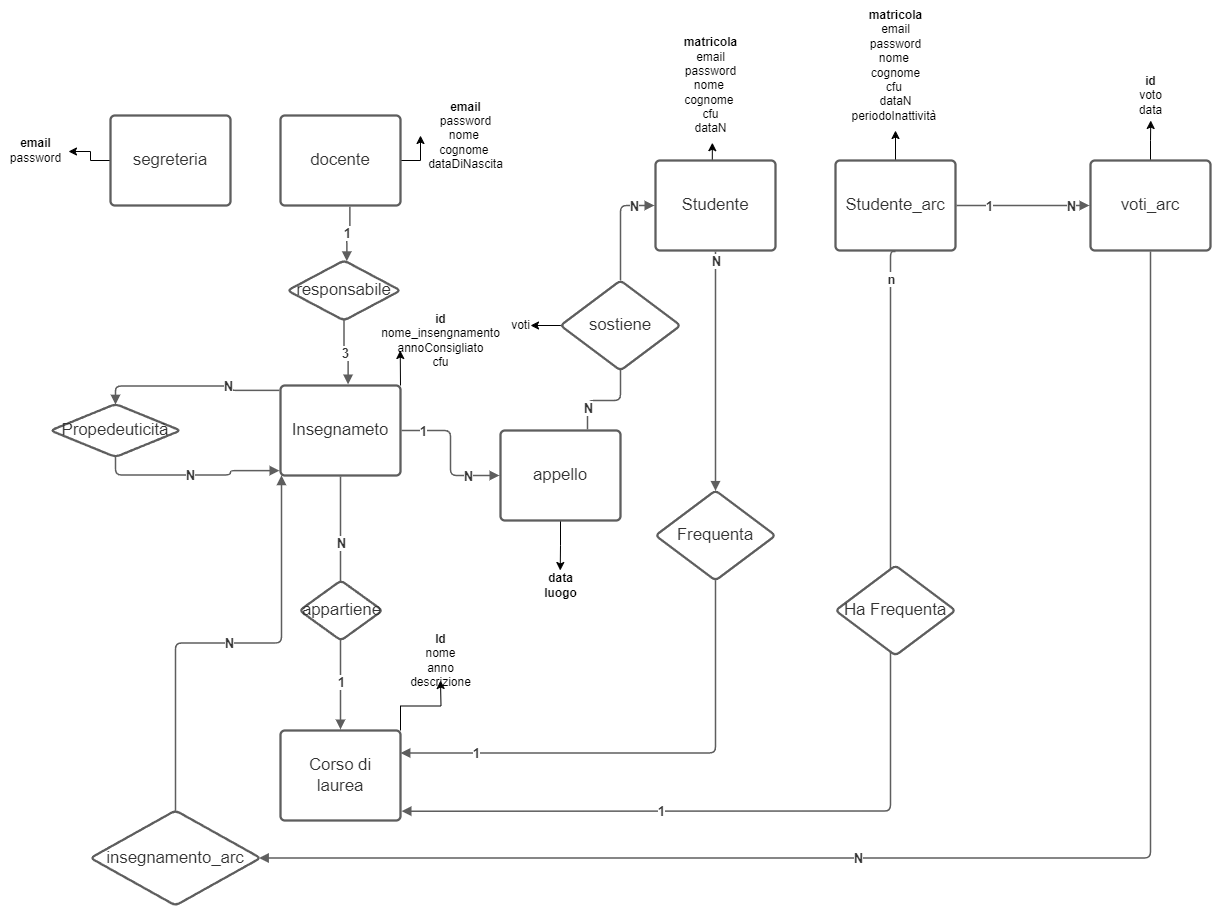
\includegraphics[width=0.8\linewidth]{images/concettuale-2.png}
    \caption{diagramma concettuale definitivo}
    \label{fig:concettuale2}
\end{figure}

Come si può notare sono state aggiunte le propedeuticità per l'insegnamento, è stata creata la relazione sostiene tra studente e appello e l'archivio è stato strutturato